\section{Suppressing the Spiders by using FFT}
We now want to use the knowledge we have gained about the Fourier transformation of different features, especially of features which resemble spiders, to suppress the signal of the spiders. The idea is to manipulate the Fourier transform of the data and then transform the data back via the inverse Fourier transformation.\\
We take the data from HD142527, warp it to the $r$-$\varphi$ plane and correct for the radial intensity drop. For the transformation we choose the radius range such that the object we want to look at is placed in the center. We choose the same radius range as in figure \ref{fig:warped_254_454} namely: $R=254-454$. In order to make sure that the aperture flux of other objects than the spiders, mainly point sources like exoplanets, is conserved we will use the ghost at radius $323$. The ghost is not perfectly in the center of the radius range, but this is not important for our purpose. The only thing which will happen, is that the aperture flux will change a bit when warping the image to the $r$-$\varphi$ plane.\\
Figure \ref{fig:rad0} shows the Fourier transform of the warped and flatten image at different radial frequencies. In contrast to the Fourier transform of the simulated spiders, the signal is not Gaussian anymore, since there are other features on top, like the ghost and the noise.
\begin{figure}[H]
	\centering
		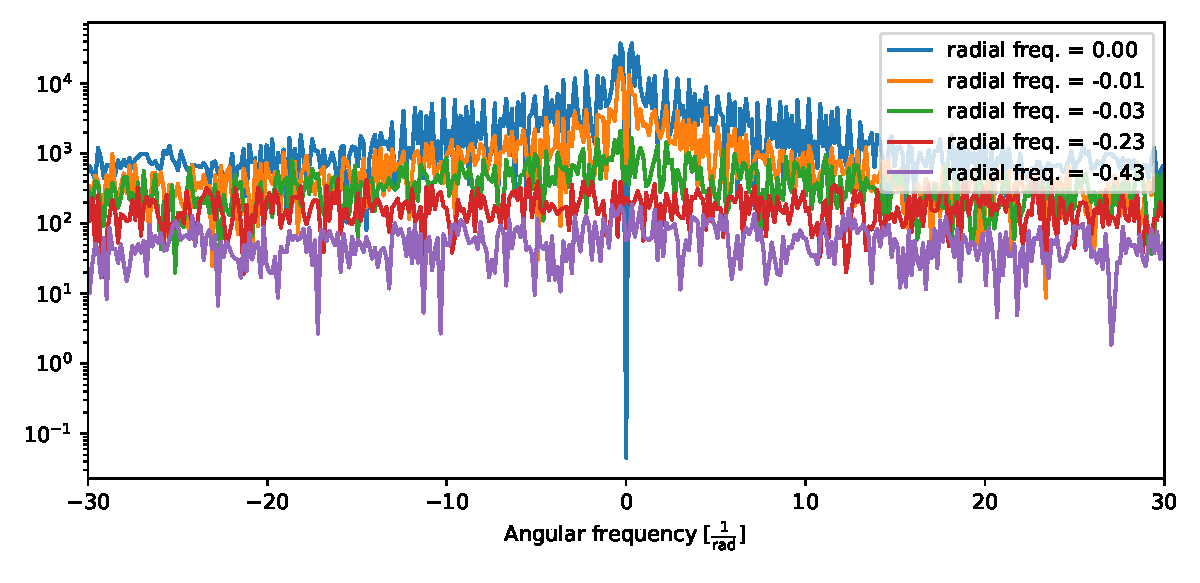
\includegraphics[width=1.0\textwidth]{pics/rad0.pdf}
		\caption{Several horizontal cuts through the frequency plane of the image data shown in figure \ref{fig:HDsuppcentralfreq_R254_R454_-0.5to0.5}(a).}
		\label{fig:rad0}
\end{figure} 

\subsection{High Frequencies}
As we saw in section \ref{sec:pointlike} the angular range in which a point-source, Gaussian or PSF, will produce a significant frequency signal is within $[-50, 50] \frac{1}{\mathrm{rad}}$ and the radial range is within $[-0.2, 0.2] \frac{1}{\mathrm{px}}$. When we consider the noise, the range is even smaller as we saw in section \ref{sec:noise}.  
Therefore we first thought it would be a good idea to suppress everything which is outside of this area by a factor of $1000$. However this is not the best idea, since the high frequencies are responsible for the edges in the image. By suppressing the high frequencies we would therefore blurry the image. This might not look like being a problem, since due to the noise the image is already blurred. As long as the point-source we look at is sufficiently large and bright this is indeed no problem, but as soon as the point-source gets fainter and smaller, it starts to disappear due to the blurring. Since we are more interested in the second case it is no option to suppress the high frequencies. Also we would not gain any positive effect through this suppression.\\
This makes us again clear that we are only looking at the absolute values of the frequency space and thus ignore big parts of the phase information as well as negative values.\\
An other attempt tried was to subtract the mean of the noisy frequency background from the whole frequency space, but this was an even badder idea. Due to the subtraction the whole back transformed image gets a weaker intensity. All structures stay unchanged, but are weaker. Like this it would be even harder to find faint structures, especially if they come too close to the numerical limits. 

\subsection{Central Radial Frequency}
\label{sec:central_radial_freq}
From our investigation of the Fourier transformation for spider-like structures, we found that their most important features are where the radial frequency is zero. Therefore, we first want to suppress the frequencies, which are caused by the spiders, at radial frequency zero.\\
As we saw in section \ref{sec:gaussian} the spiders produce a signal in the frequency plane, especially for radial frequency equals zero, which is close to a Gaussian. We divide our central radial frequency by the Gaussian profile with width $\sigma = 8.7 \frac{1}{\mathrm{rad}}$, which we found from our simulations of the spiders, see figure \ref{fig:simspi_noise_angularfreq}. By doing this we ignore the fact that we have some oscillations on top of the true signal. To reassure that this approximation is appropriate we compare the resulting back-transformed images after a division by the Gaussian profile and after a division by the Fourier transform at radial frequency zero which we get from our simulations. From the comparison we find that the Gaussian profile is a really good approximation, since by eye we cannot see any differences between the resulting back-transformed images and also the aperture fluxes of the ghosts are almost the same. We also computed the aperture flux of a PSF which we placed on the image far away from the spiders and also this aperture flux was almost the same, also for different intensities of the PSF.\\
As a next step we want to find out in which angular range around the central frequency we need to divide by the Gaussian. This is a really important parameter, since if the angular width is so large, that the value of the Gaussian profile at this position is smaller than one. The division will lead to an increase of the intensity instead of a suppression. Figure \ref{fig:rad0_diffsubwidths} shows the aperture flux of the ghost after the division by a Gaussian at radial frequency zero for different angular frequency ranges around zero. The orange line marks the aperture flux of the ghost after the warping and the correction for the radial drop-off, we call it the initial aperture flux. Whereas the blue dots mark the aperture flux of the ghost after the division by the Gaussian for different angular widths.\\
Since it is even an advantage, if the aperture flux increases through the procedure, we choose the width with which we get the largest aperture flux, which is the case for $9.1 \frac{1}{\mathrm{rad}}$. This means we divide by the Gaussian in the following angular range: $[-9.1, 9.1] \frac{1}{\mathrm{rad}}$. An increase of the aperture flux is really good, because it means that the spiders are being suppressed without suppressing the ghost. Ghost 2, at which we are looking, is a good indicator for this, because in this image he is situated close to a spider.
\begin{figure}[H]
	\centering
		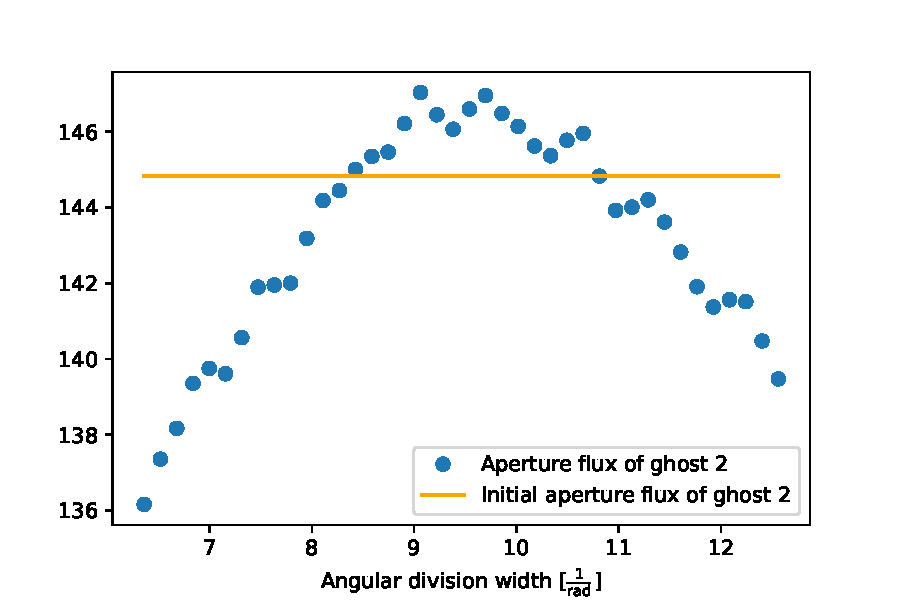
\includegraphics[width=1.0\textwidth]{pics/rad0_diffsubwidths.pdf}
		\caption{For radial frequency zero the Fourier transform of the image data is divided by a Gaussian which has its center at angular frequency zero. The division is not performed along the complete angular range, but only for a certain width around zero. We have plotted the aperture flux of ghost 2 for different angular division widths. The width which produces the largest flux is ideal.}
		\label{fig:rad0_diffsubwidths}
\end{figure}
Other parameters of this suppression are the intensity and the width of the Gaussian profile. We find that the resulting back-transformed image is not at all sensible on this variables. This is due to the fact that we divide by the Gaussian and do not subtract by it. It is not such a problem if we divide everything by $10^4$ or by $10^3$. Actually a subtraction would be mathematically more correct, but the subtraction is highly sensible on every single parameter and a division is a lot more stable. Also when dividing we can only look at the absolute values of the Fourier transform, but when subtracting we would have to take into account also the negative values. An other reason for the insensibility on the width of the Gaussian profile is that we only look at a narrow angular range, where the width of the Gaussian profile does not have a big influence. \\
Figure \ref{fig:HDsuppcentralfreq_R254_R454_-0.5to0.5}(a) shows the warped and flatten image from $R=254-454$ and its Fourier transform. In figure \ref{fig:HDsuppcentralfreq_R254_R454_-0.5to0.5}(b) the Fourier transform at radial frequency zero in the above defined angular range is divided by the Gaussian profile and its back-transformed image are shown. To get back into the $r$-$\varphi$ plane we use the inverse Fourier transformation. When we compare the image before and after the Gaussian division we can already observe that the spiders are a lot less bright. Especially around the central radius the results is really good. This is for us the most important region, since this is also the region where the object we are interested in, will be. Below the central radius the spiders almost stay the same or change only slightly and above the central radius we have a trend to the other extreme, meaning we have negative values. We also observe that the noise gets weaker and is smoother distributed.\\
From the steps we have made so far the aperture flux increases by $6.64$ \% compared to the initial aperture flux for ghost 2 and by $49.73$ \% for the PSF, here we use a PSF which is approximately $10^{-6}$ times less bright then the star. 
\begin{figure}[H]
	\centering
		\subfigure[]{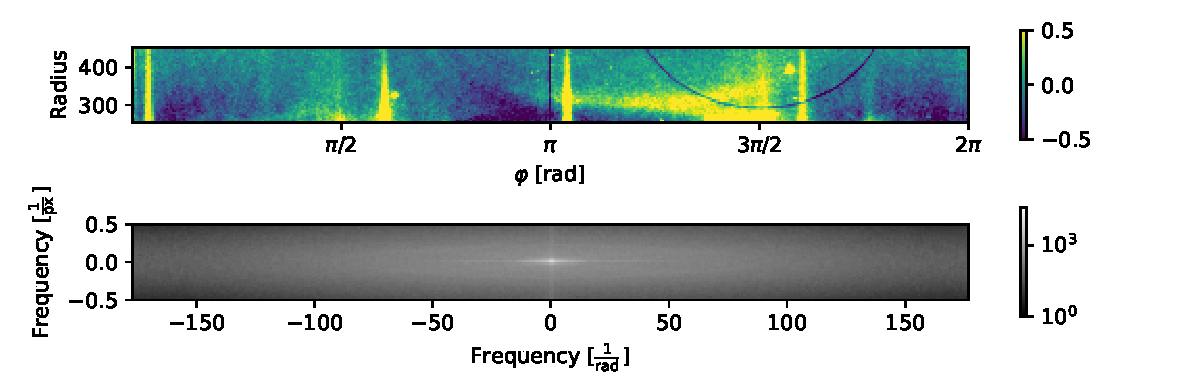
\includegraphics[width=1.1\textwidth]{pics/HDflatten_R254_R454_-0.5to0.5.pdf}}
		\subfigure[]{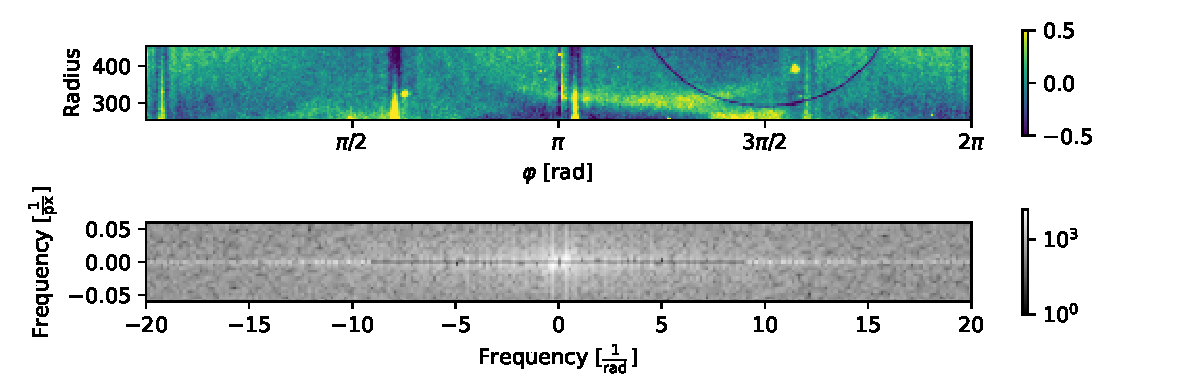
\includegraphics[width=1.1\textwidth]{pics/HDsupprcentralfreq_R254_R454_-0.5to0.5.pdf}}
\caption{An image from HD142527 which has been warped to the $r$-$\varphi$ plane and flattened and its Fourier transform (a). After a division of the central frequencies at radial frequency zero by a Gaussian profile, the spider in the back-transformed image are less bright (b).}
\label{fig:HDsuppcentralfreq_R254_R454_-0.5to0.5}
\end{figure}

\subsection{Low Frequencies}
As we saw during the simulation of the spiders, not only the frequencies at radial frequency zero have non-zero values, but there is also an extension into the radial frequencies which are unequal to zero. In the following we will also suppress the frequencies which are cause by the spiders in this regime. But due to the noise level, the interesting radial regime only goes until approximately $[-0.06, 0.06] \frac{1}{\mathrm{px}}$. As we already discussed in section \ref{sec:central_radial_freq} the regime is even smaller, since we need to avoid to divide through values which are smaller than one. The same holds for the angular range. The angular range is smaller for larger absolute radial frequency values, since the intensity of the complete signal is overall smaller. In conclusion we will only be able to suppress the lowest frequencies.\\
First of all we have to choose a Gaussian profile with an adequate width and intensity. As before when we suppressed the central radial frequency, we choose the Gaussian profiles such that it best fits to the signal of our spider simulation. For the signal at radial frequency $-0.005$/$0.005 \frac{1}{\mathrm{px}}$ (this is the are the two ones closest to the radial frequency center and they are the same due to the symmetry of the Fourier transform) we choose a Gaussian profile with width $\sigma_s = 6.4 \frac{1}{\mathrm{rad}}$ and intensity $I_s = 0.84 I = 8.4 \cdot 10^3$ where $I$ is the intensity of the Gaussian profile used for suppressing the frequencies at radius zero. As before the width and the intensity of the Gaussian profile are not so important for the suppression and does not matter if they differ a bit. But the angular frequency width $w_s$ in which we do the division (as in section \ref{sec:central_radial_freq}) as well as the radial frequency width $h$ is essential.\\
To find these two parameters we use the same procedure we used to find the angular frequency width $w$ for radial frequency zero. Namely we try out different parameters and take the one with which we get the largest aperture flux for ghost 2. As before we will also use a second object in form of a PSF which is placed not in the surrounding of one of the spiders, in order to check that the procedure really does what we want. The PSF is approximately $10^{-6}$ times less bright then the star. We find that $h = 0.01 \frac{1}{\mathrm{px}}$ and $w_s = 7.2 R \frac{1}{\mathrm{rad}}$, where $R$ is the ratio between the mean central radial frequency (considering only low angular frequencies) and the mean radial frequency in which the division is taking place.\\
The parameters for the other radial frequencies with an absolute value which is larger than $0.005 \frac{1}{\mathrm{px}}$, but still smaller than $h$, are derived from the one at absolute radial frequency $0.005 \frac{1}{\mathrm{px}}$. In figure \ref{fig:simspi_angularfreq} we observed that the non-central low radial frequencies all have the same shape, but different intensities. Therefore we choose the same Gaussian profile for all of them and multiply it with a the factor $R$.\\
Figure \ref{fig:HDsupplowfreq_R254_R454_-0.5to0.5.pdf} shows the image from HD142527 after the suppression of the low frequencies as discussed before and the suppression of the central radial frequency. We observe that now the overall brightness of each spider from figure \ref{fig:HDsuppcentralfreq_R254_R454_-0.5to0.5} to figure \ref{fig:HDsupplowfreq_R254_R454_-0.5to0.5.pdf} has not changed significantly, but the gradient from low to larger radius which we had before has almost completely vanished. Also the whole image is a lot smoother. This can also be observed in the aperture fluxes. As ghost 2 is placed near a spider and is almost in the center of the radial range, its aperture flux is almost the same as after the suppression of the central radial frequency only and so the aperture flux increased by $6.74$ \% compared to its initial aperture flux. Whereas the aperture flux of the PSF increased by $53.12$ \%. 
\begin{figure}[H]
	\centering
		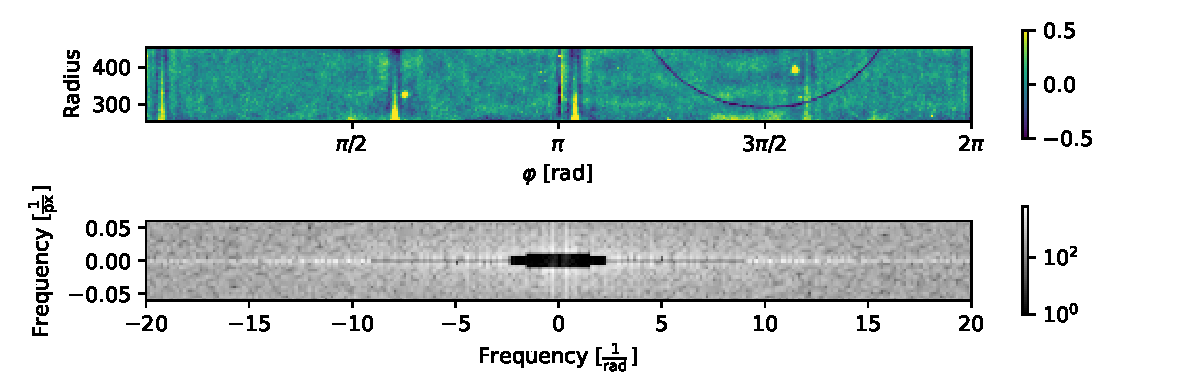
\includegraphics[width=1.1\textwidth]{pics/HDsupplowfreq_R254_R454_-0.5to0.5.pdf}
		\caption{The image from HD142527 after the central radial frequency and the low frequency are suppressed in the frequency plane and transformed back to the image plane via inverse Fourier transformation.}
		\label{fig:HDsupplowfreq_R254_R454_-0.5to0.5.pdf}
\end{figure}

\subsection{Results}
To verify that our suppression of the spider through Gaussian division does not only work on the single data we have used until now. We perform the suppression on different images of HD142527. The data is taken in P2-mode, in this mode the ghosts and the possible exoplanets do not wander, but the spiders do. 


Differences: Images have different intensities -> angular division width needs to be adapted to the overall intensity -> Is it not really worth it, since the results are not really great